\begin{appendices}
\section{}\label{sec:appendix}
\begin{figure}[h]
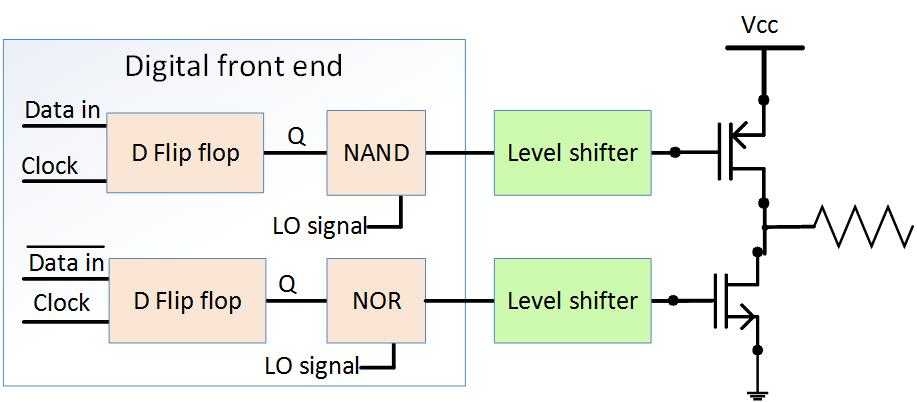
\includegraphics[width=0.5\textwidth]{Global_schematic_previous_group.jpg}
\caption{Global schematic of the previous group.}
\label{fig:Global_schematic_previous_group_figure}
\end{figure}

\begin{figure}[h]
 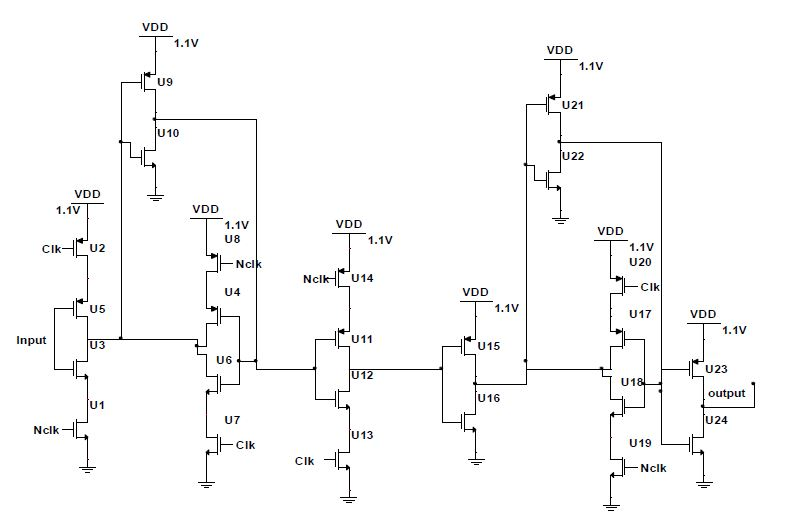
\includegraphics[width=0.5\textwidth]{D_flip_flop_schematic.jpg}
 \caption{ D flip flop schematic from previous group}
 \label{fig:D_flip_flop_ previous_group_figure}
\end{figure}

\begin{figure}[h]
 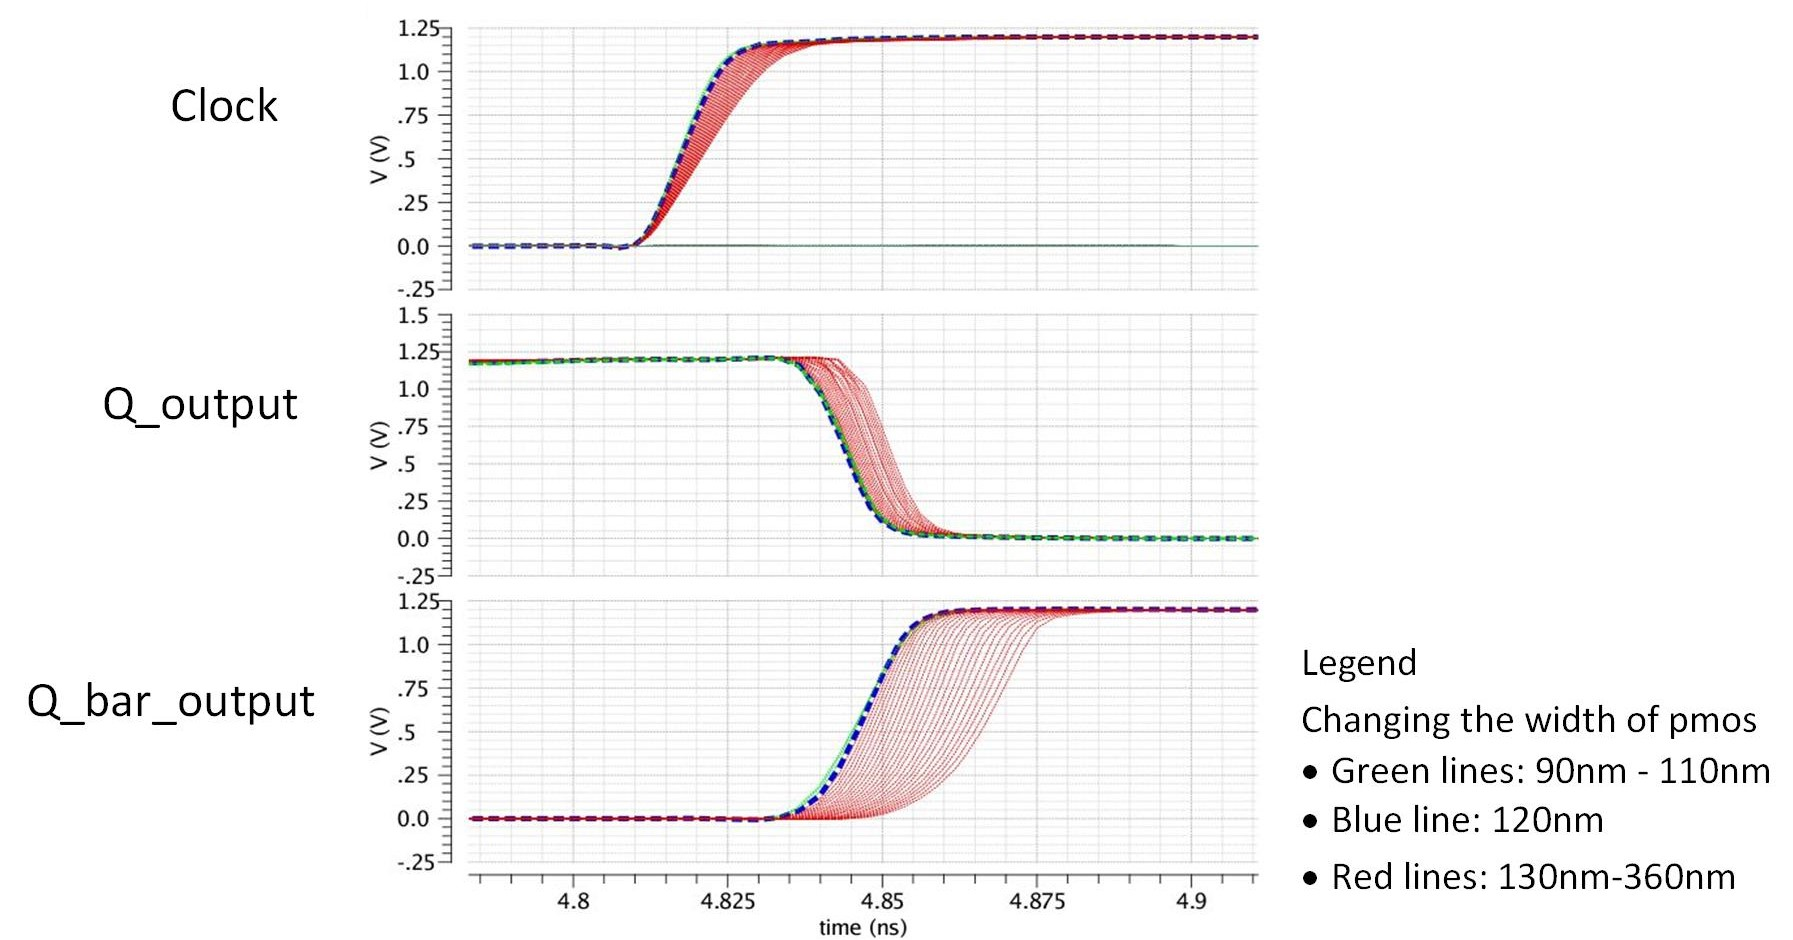
\includegraphics[width=0.5\textwidth]{Parameter_sweep_changing_w_high_to_low.jpg}
 \caption{Parametersweep of changing the width of the pmos when the data is low.}
 \label{fig:parametersweep_changing_w_high_to_low_figure}
\end{figure}

\begin{figure}[h]
 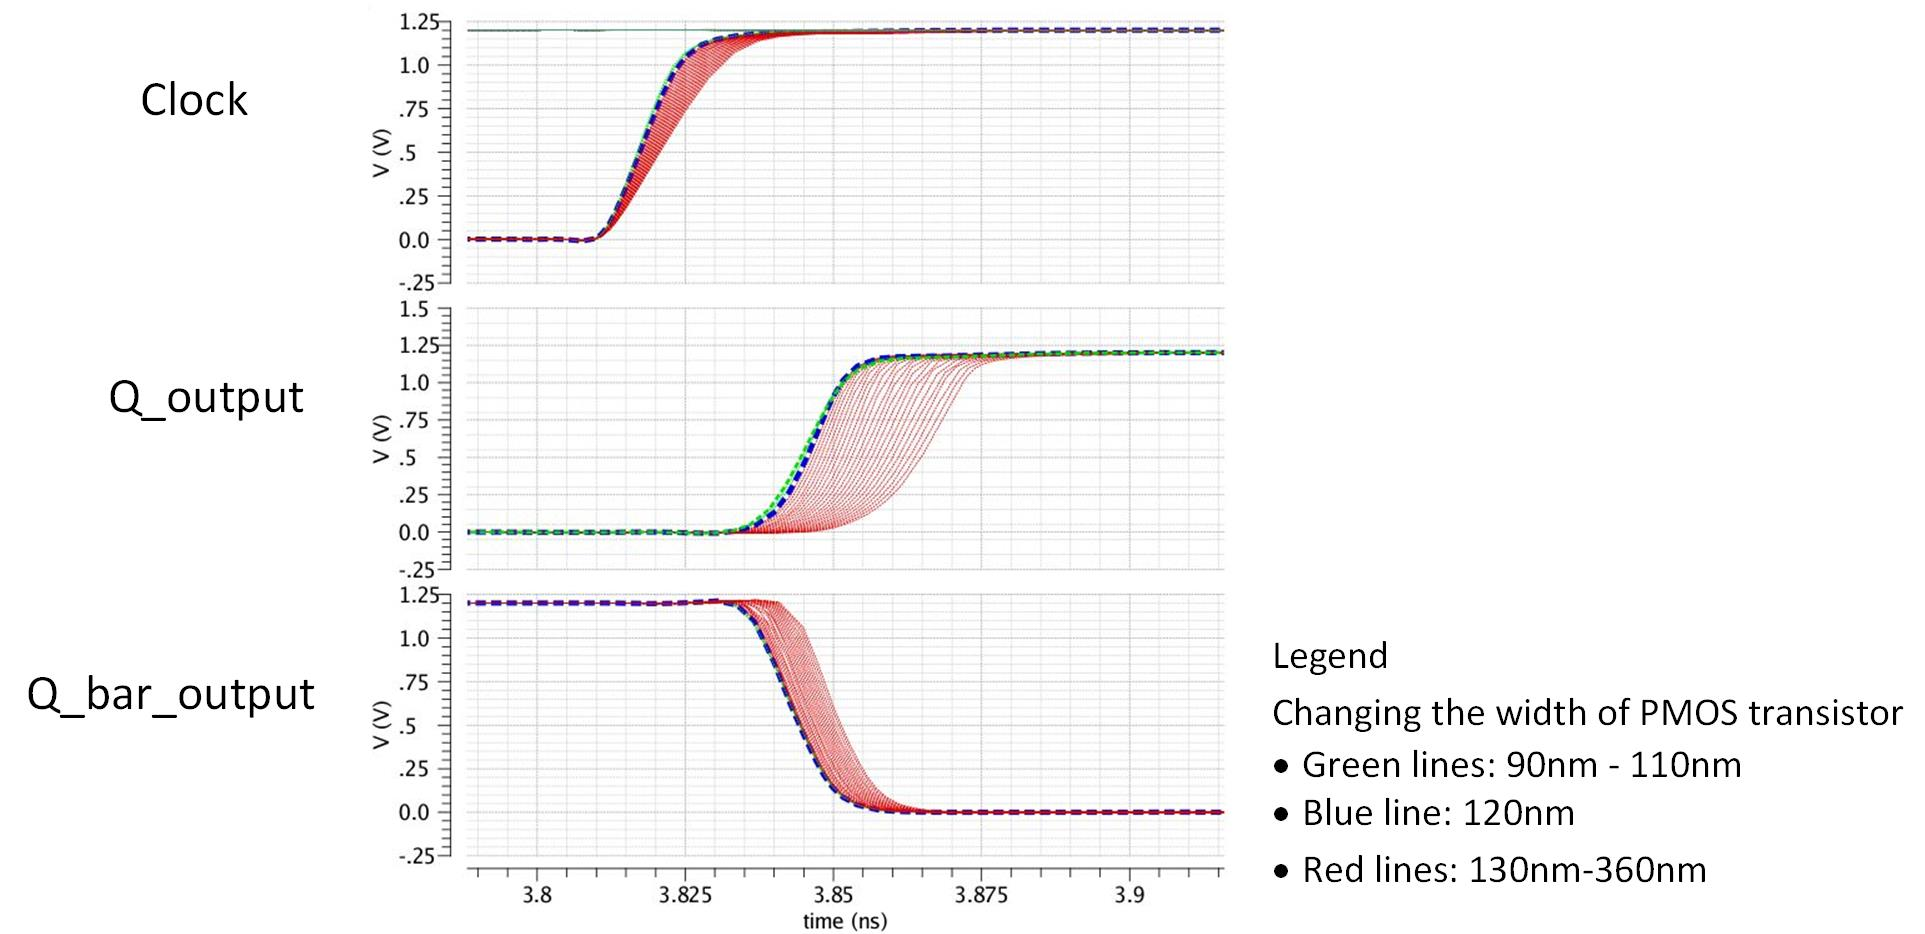
\includegraphics[width=0.5\textwidth]{Parameter_sweep_changing_w_low_to_high.jpg}
 \caption{Parametersweep of changing the width of the pmos when the data is high.}
 \label{fig:parametersweep_changing_w_low_to_high_figure}
\end{figure}

\begin{figure}[h]
 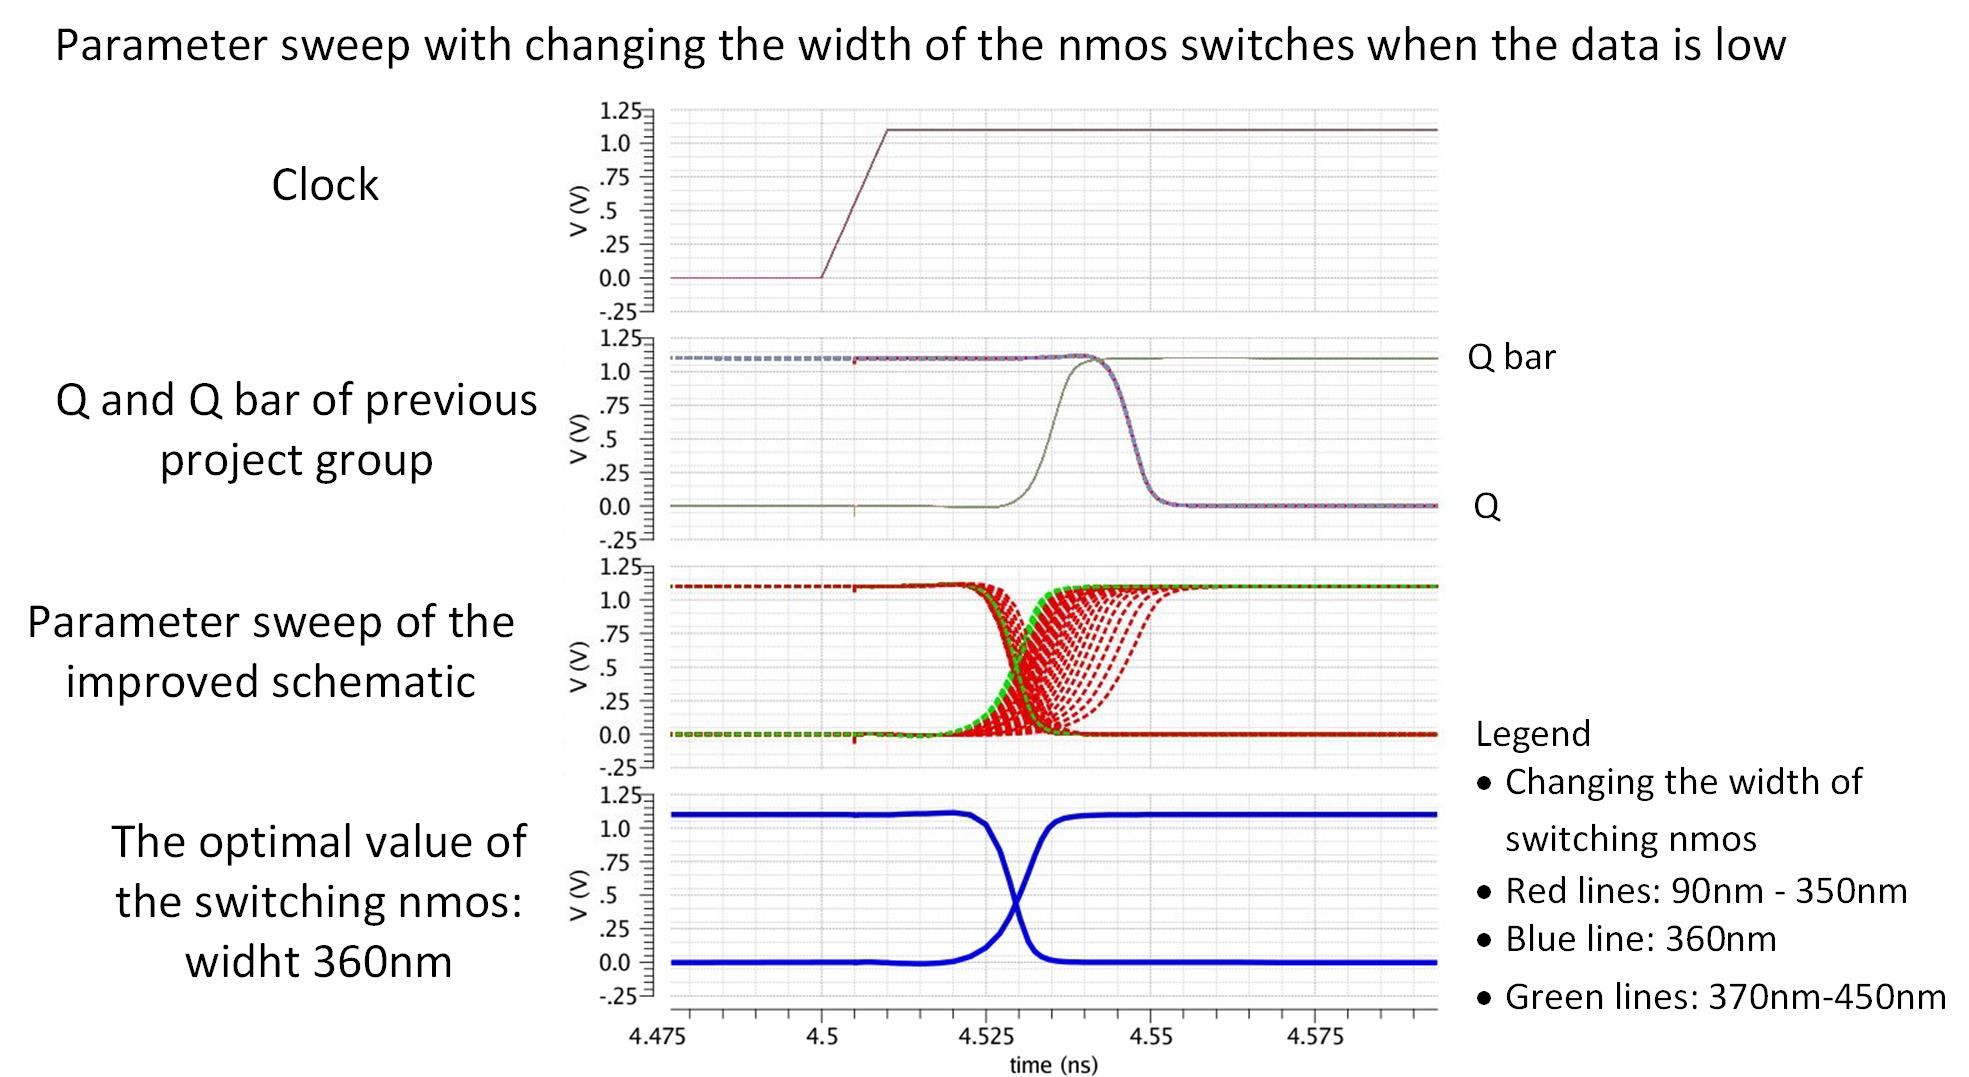
\includegraphics[width=0.5\textwidth]{Parameter_sweep_changing_w_of_the_swiching_nmos_high_to_low.jpg}
 \caption{Parameter sweep of changing the width of the switching nmos when the data is low.}
 \label{fig:Parameter_sweep_changing_w_of_the_swiching_nmos_high_to_low_figure}
\end{figure}

\begin{figure}[h]
 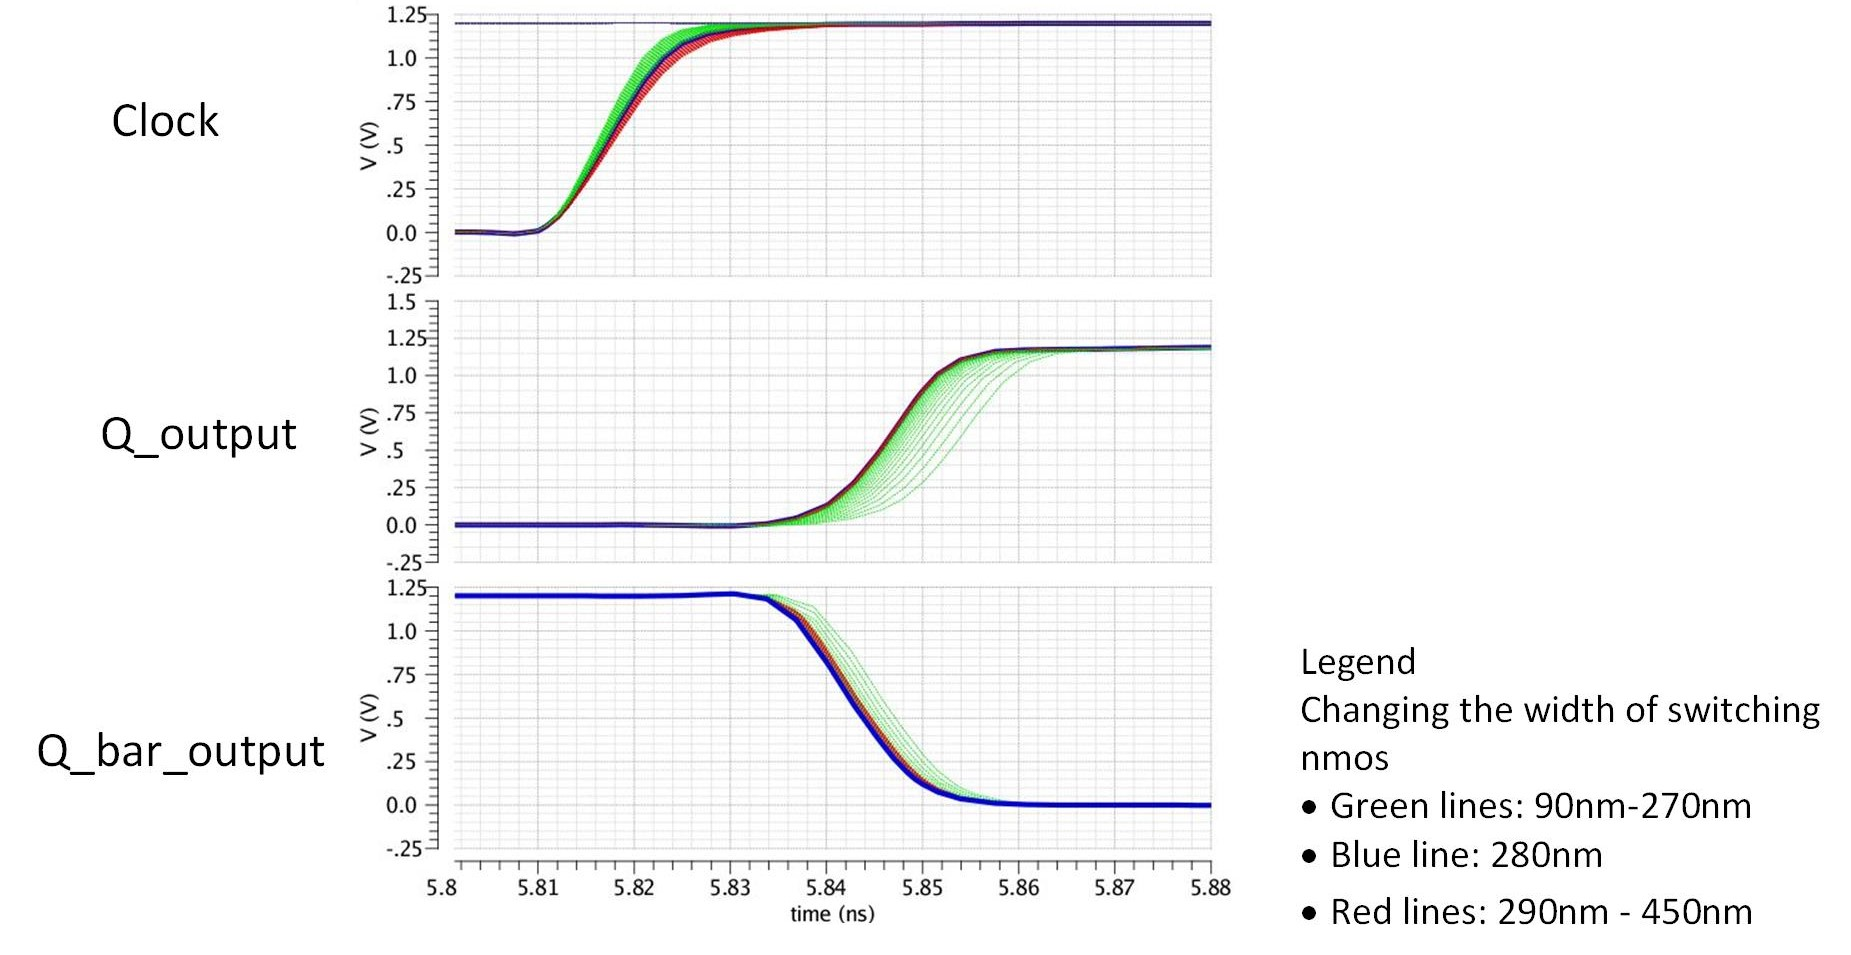
\includegraphics[width=0.5\textwidth]{Parameter_sweep_changing_w_of_the_swiching_nmos_low_to_high.jpg}
 \caption{Parameter sweep of changing the width of the switching nmos when the data is high}
 \label{fig:Parameter_sweep_changing_w_of_the_swiching_nmos_low_to_high_figure}
\end{figure}

\begin{figure}[h]
 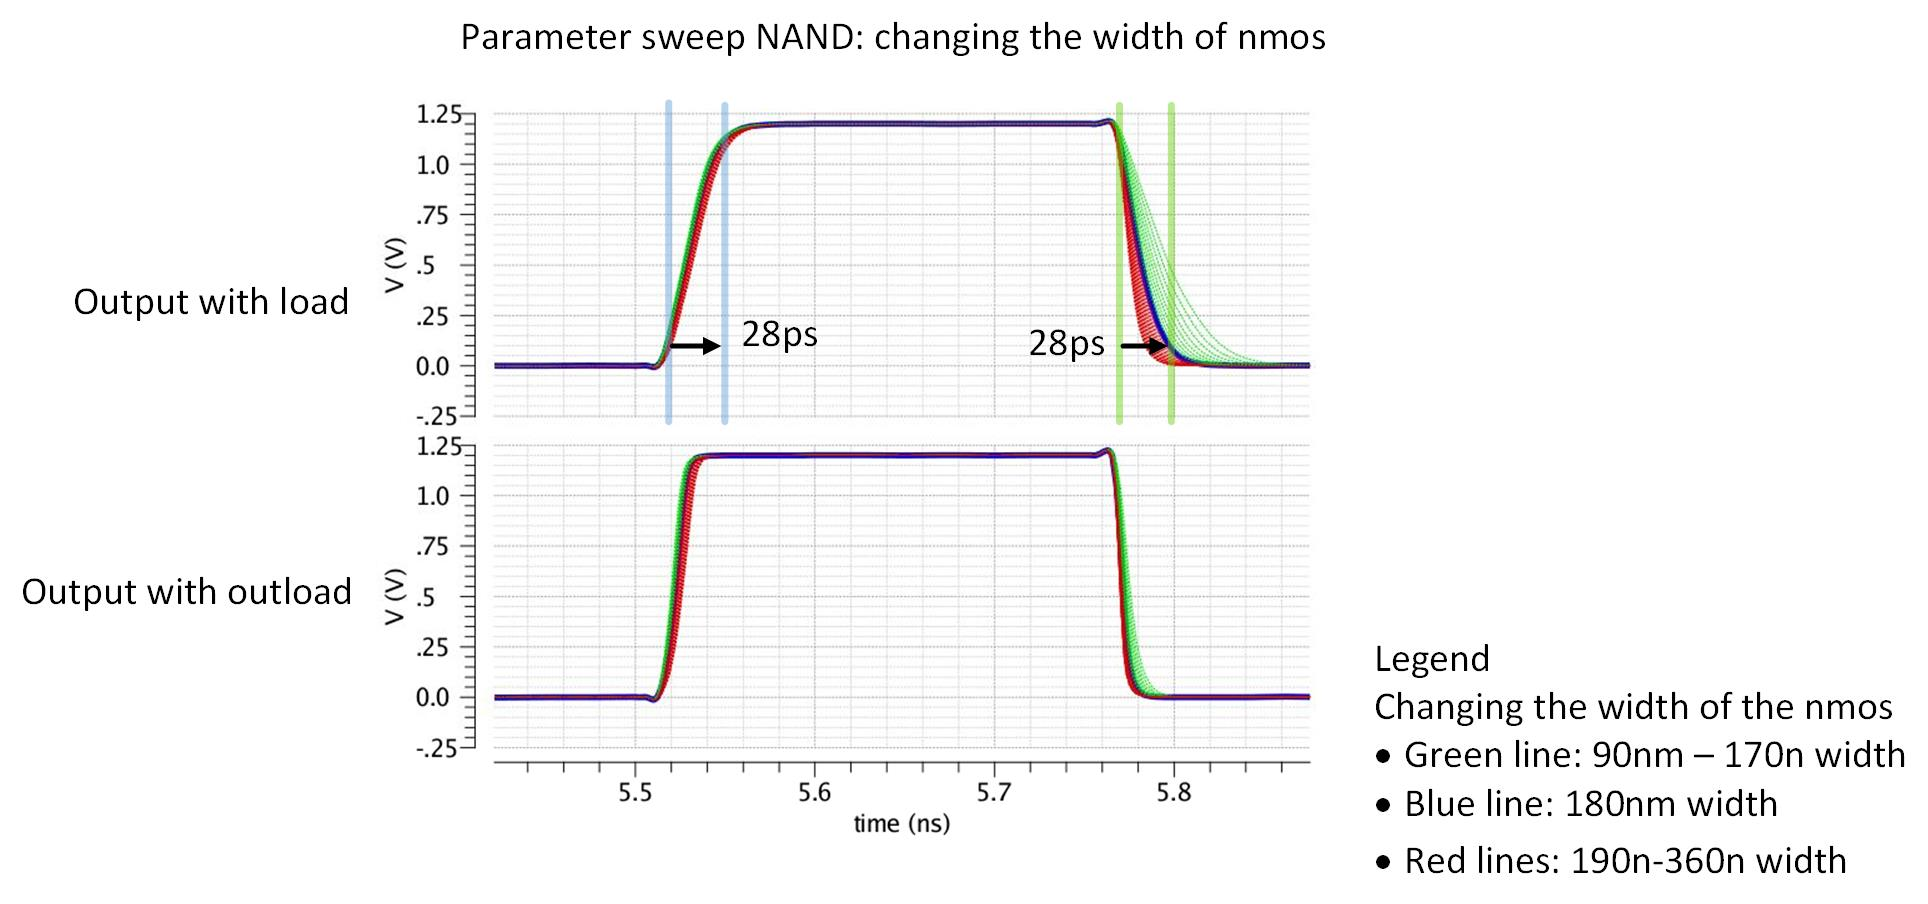
\includegraphics[width=0.5\textwidth]{NAND_nmos_sweep.jpg}
 \caption{Parameter sweep of changing the width nmos of the NAND.}
 \label{fig:NAND_nmos_sweep_figure}
\end{figure}

\begin{figure}[h]
 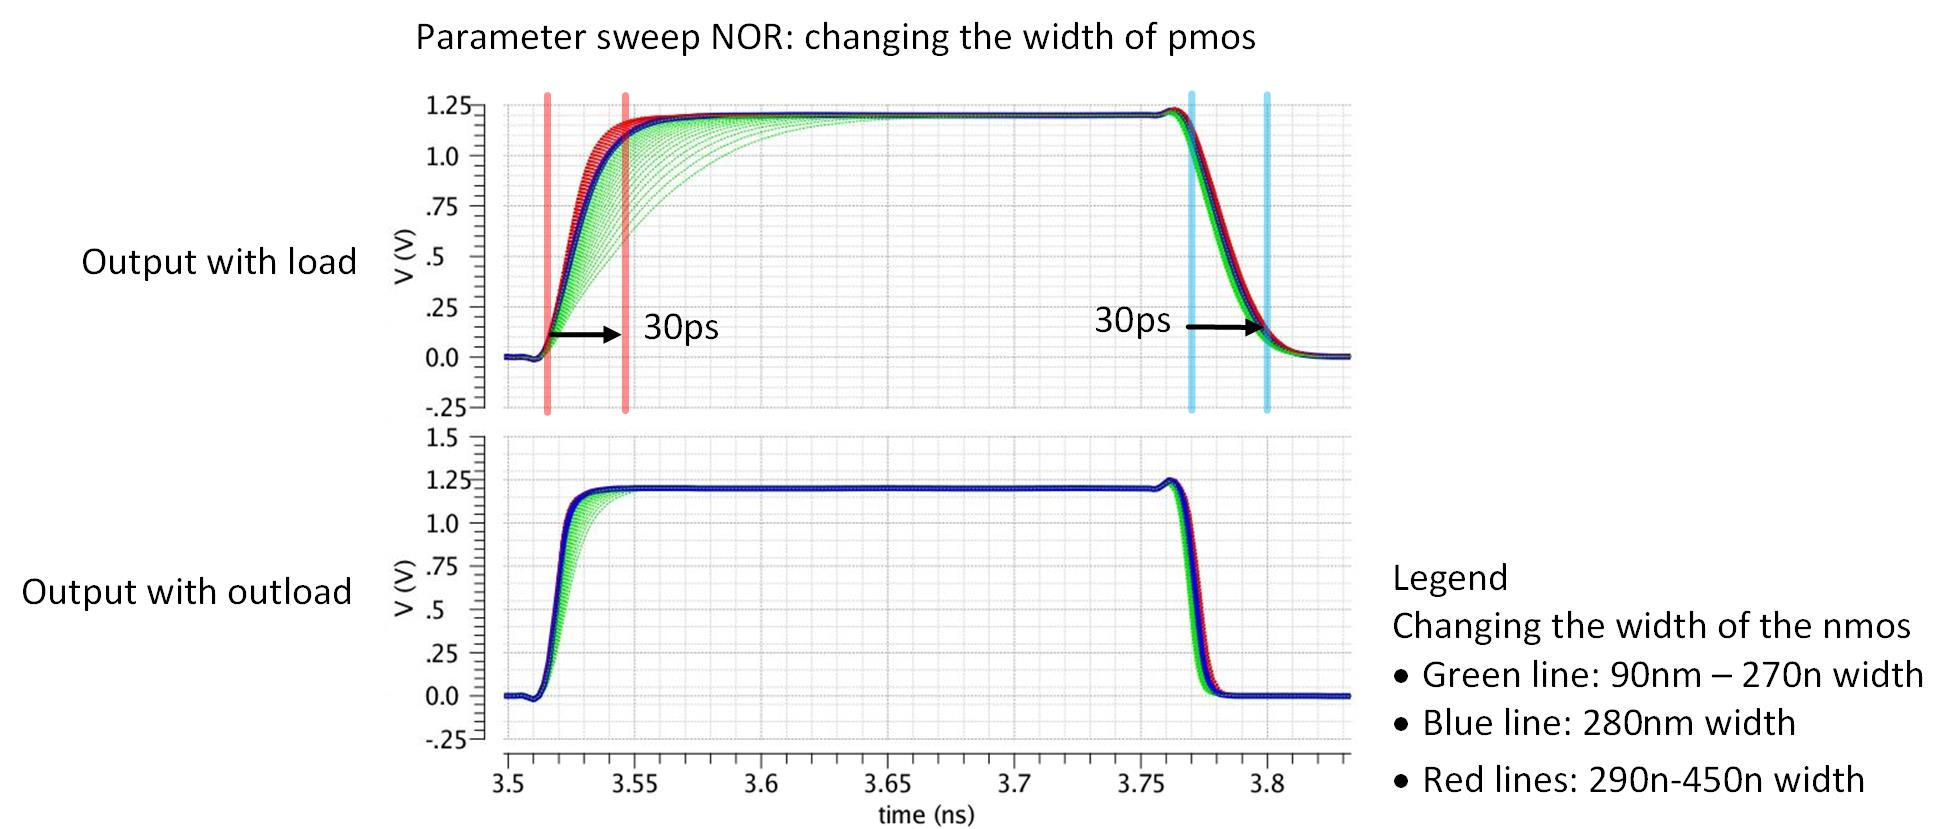
\includegraphics[width=0.5\textwidth]{NOR_pmos_sweep.jpg}
 \caption{Parameter sweep of changing the width pmos of the NOR.}
 \label{fig:NOR_pmos_sweep_figure}
\end{figure}

\begin{table}[h!]
\caption{This table lists the dimensions of the transistors in the levelshifter that drives the PMOS current sources.}
\begin{tabular}{l||l|l}\arraybackslash
Transistor & Width(um) & Length (nm) \\\hline\hline
M1 & 20 & 200\\\hline
M2 & 60 & 200\\\hline
M3 & 10 & 350\\\hline
M4 & 10 & 350\\\hline
M5 & 1.2 & 50\\\hline
M6 & 1.2 & 50
\end{tabular}
\label{Tab:Levelshifter_PMOS_sizes}
\end{table}

\begin{table}[h!]
\caption{This table lists the dimensions of the transistors in the levelshifter that drives the NMOS current sources.}
\begin{tabular}{l||l|l}\arraybackslash
Transistor & Width(um) & Length (nm) \\\hline\hline
M1 & 20 & 200\\\hline
M2 & 60 & 200\\\hline
M3 & 10 & 350\\\hline
M4 & 10 & 350\\\hline
M5 & 1.2 & 50\\\hline
M6 & 1.2 & 50\\\hline
M7 & 50 & 1700\\\hline
M8 & 20 & 200
\end{tabular}
\label{Tab:Levelshifter_NMOS_sizes}
\end{table}

\begin{table}[h!]
\caption{This table describes which widths and lengths are used for which NMOS transistors. M1 is the MOSFET which is associated with the lowest current while M15 is associated with the highest current.}
\begin{tabular}{l||l|l}\arraybackslash
NMOS & Width(um) & Length (um) \\\hline\hline
M1 & 30.00 & 0.9\\\hline
M2 & 30.17 & 0.9\\\hline
M3 & 30.30 & 0.9\\\hline
M4 &  30.30 & 0.9\\\hline
M5 & 30.36 & 0.9\\\hline
M6 & 30.44 & 0.9\\\hline
M7 & 30.49 & 0.9\\\hline
M8 & 30.57 & 0.9\\\hline
M9 & 30.66 & 0.9\\\hline
M10 & 30.74 & 0.9\\\hline
M11 & 30.83 & 0.9\\\hline
M12 & 30.95 & 0.9\\\hline
M13 & 31.05 & 0.9\\\hline
M14 & 31.18 & 0.9\\\hline
M15 & 31.33 & 0.9
\end{tabular}
\label{Tab:NMOS}
\end{table}
\begin{table}
\caption{This table describes which widths and lengths are used for which PMOS transistors. M1 is the MOSFET which is associated with the lowest current while M15 is associated with the highest current.} 
\begin{tabular}{l||l|l}
PMOS & Width(um) & Length (um) \\\hline\hline
M1 & 56.23 & 0.3\\\hline
M2 & 57.25 & 0.3\\\hline
M3 & 57.63 & 0.3\\\hline
M4 & 57.84& 0.3\\\hline
M5 & 58.04 & 0.3\\\hline
M6 & 58.28 & 0.3\\\hline
M7 & 58.56 & 0.3\\\hline
M8 & 58.87 & 0.3\\\hline
M9 & 59.21 & 0.3\\\hline
M10 & 59.57 & 0.3\\\hline
M11 & 59.95 & 0.3\\\hline
M12 & 60.36 & 0.3\\\hline
M13 & 60.82 & 0.3\\\hline
M14 & 61.31 & 0.3\\\hline
M15 & 61.87 & 0.3
\end{tabular}
\label{Tab:PMOS}
\end{table}

\begin{figure}[htp] 
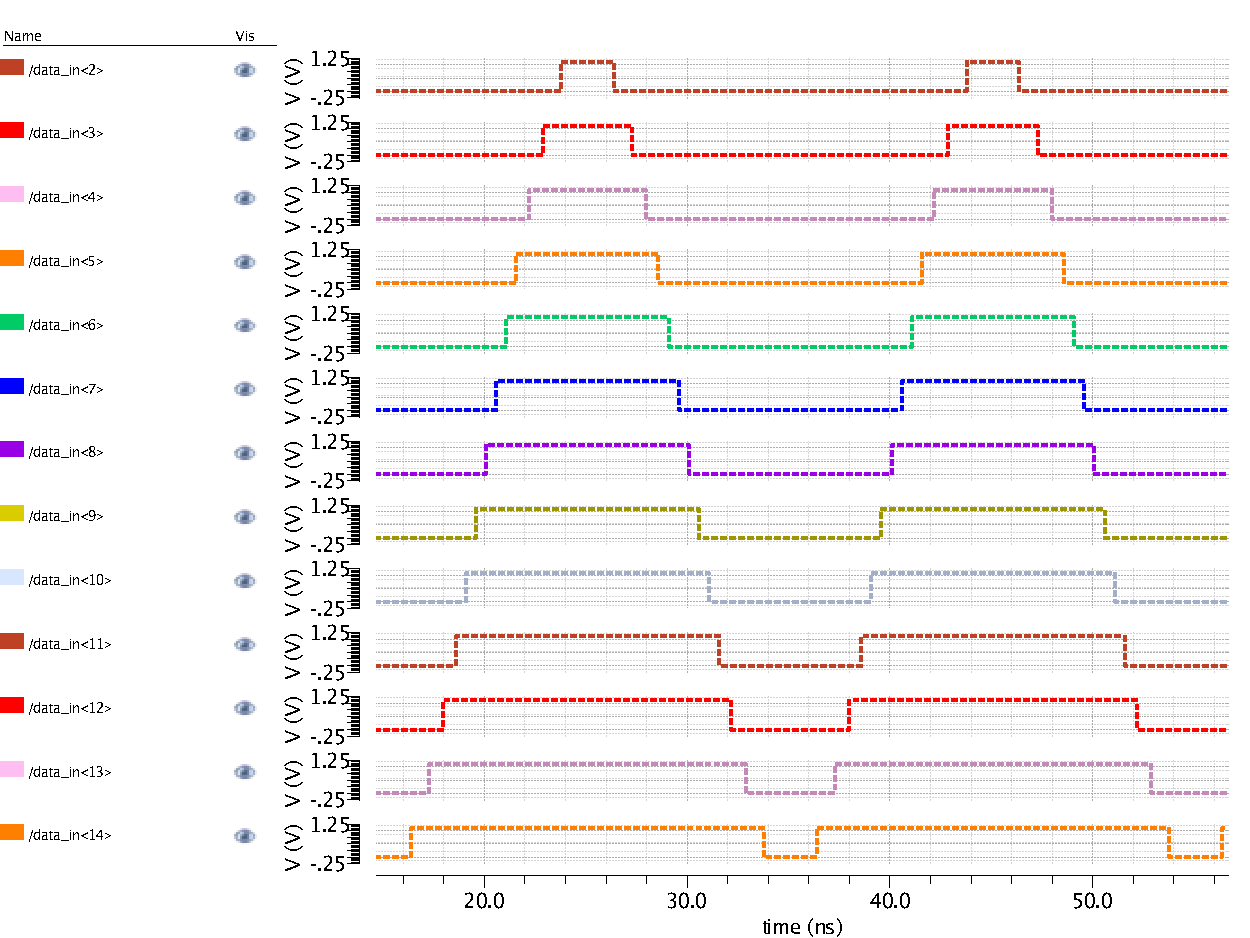
\includegraphics[width=0.5\textwidth]{thermometer_output.pdf}
\caption{Thermometer single tone voltage output.}
\label{fig:Thermometer}
\end{figure}

\begin{figure}[htp] 
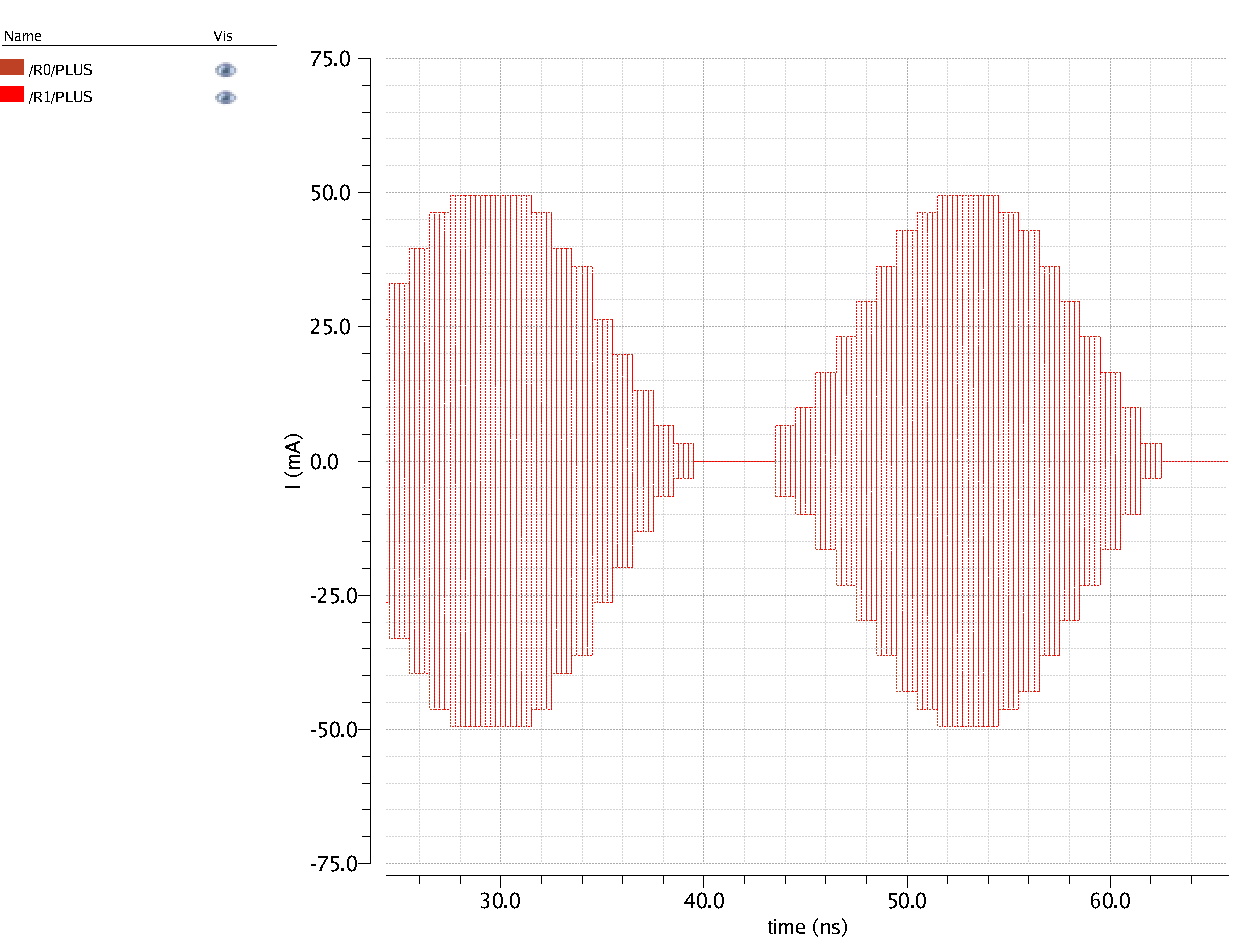
\includegraphics[width=0.5\textwidth]{Iout_ideal.pdf}
\caption{Output current}
\label{fig:Output current}
\end{figure}

\begin{figure}[htp] 
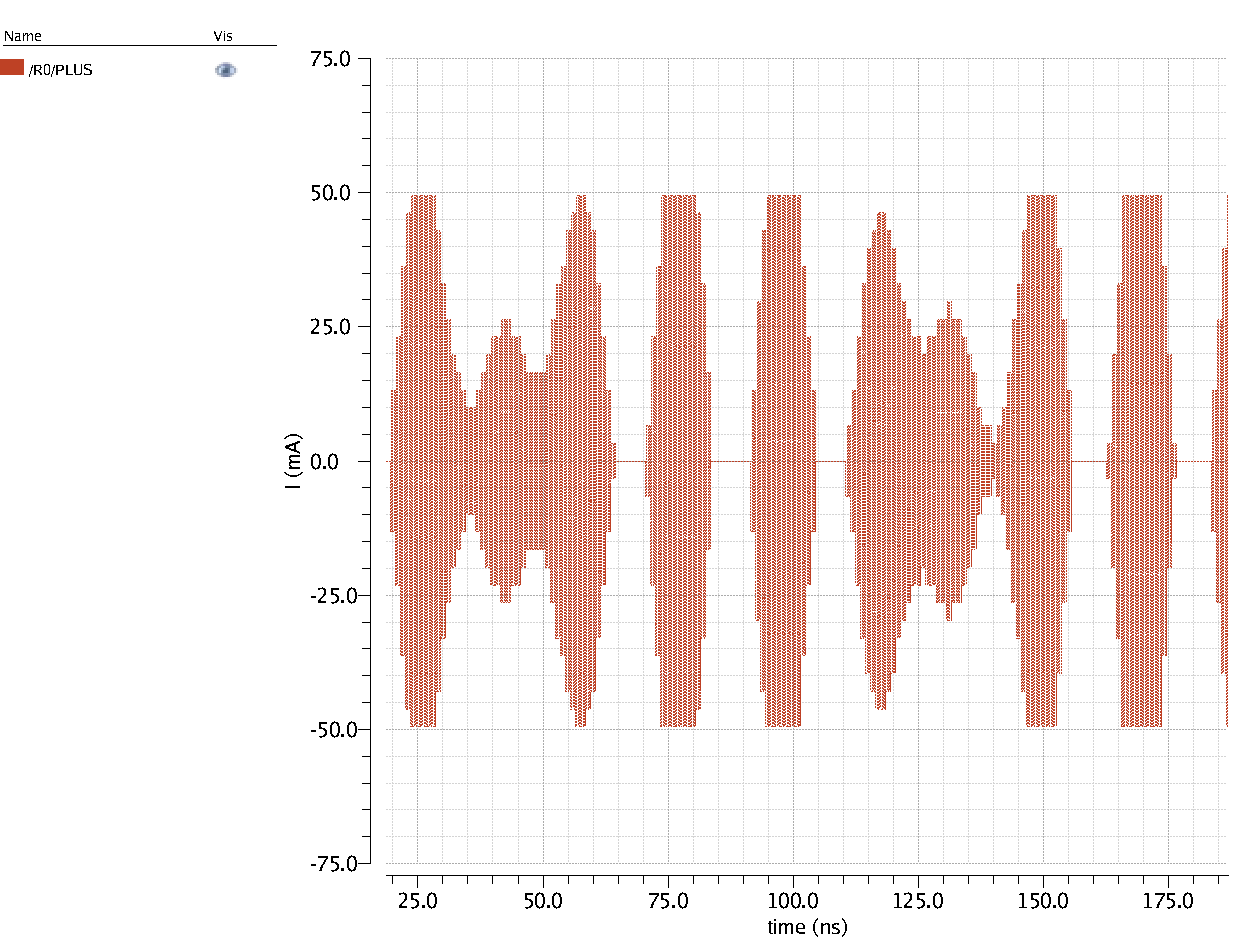
\includegraphics[width=0.5\textwidth]{trans_two_tone.pdf}
\caption{Two tone output current}
\label{transient_two_tone}
\end{figure}
\end{appendices}